\begin{lstlisting}
p159 4 5 9
\end{lstlisting}
\begin{exercise}
\begin{figure}[H]
\centering
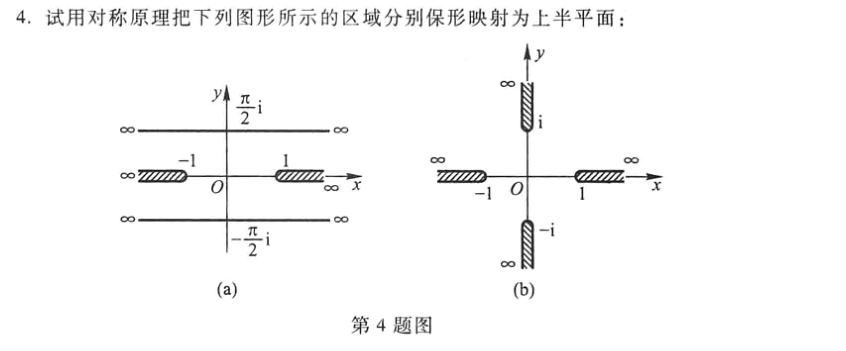
\includegraphics[width=\textwidth]{hw15-2025060920.png}
% \caption{}
\label{}
\end{figure}
\end{exercise}
\begin{theorem}[\textbf{对称原理} (或反射原理)]
设区域 $D$ 在实轴的上方,其边界 $\partial D$ 包含实轴上的一个开区间 $I$. 设函数 $f(z)$ 在 $D$ 内解析,并且在 $I$ 上连续且取实数值. 则 $f(z)$ 可以延拓到区域 $D \cup I \cup D^*$ (其中 $D^* = \{z^* : z \in D\}$, $z^*$ 表示 $z$ 的共轭复数) 上成为一个解析函数 $\widehat{f}(z)$,并且对于任意 $z \in D \cup I \cup D^*$,有 $\widehat{f}(z^*) = (\widehat{f}(z))^*$. 特别地,当 $z \in D$,我们有 $f(z^*) = (f(z))^*$.
\end{theorem}
\begin{figure}[H]
\centering
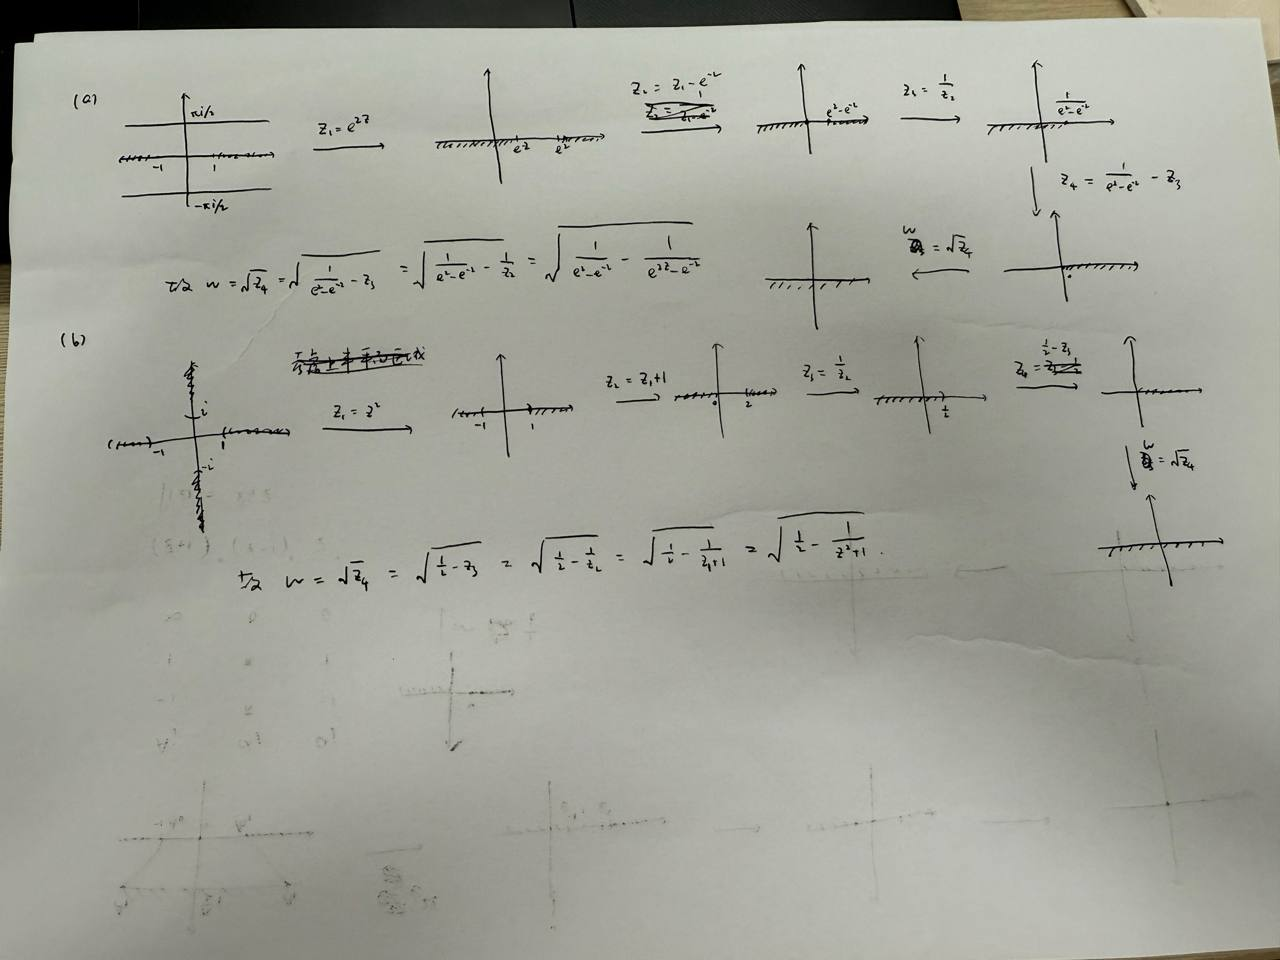
\includegraphics[width=\textwidth]{hw15-2025061010.png}
% \caption{}
\label{}
\end{figure}

\begin{exercise}
\begin{figure}[H]
\centering
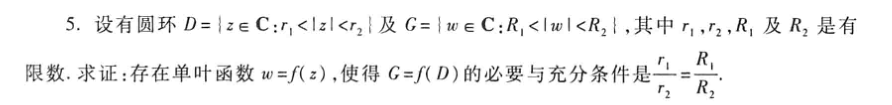
\includegraphics[width=\textwidth]{1-hw15-2025060920.png}
% \caption{}
\label{}
\end{figure}
\end{exercise}
若 $\frac{r_1}{r_2}=\frac{R_1}{R_2}$,那么可以取单叶函数 $f(z)=z\cdot\frac{r_1}{R_1}$. 考虑微分同胚 $a:z\mapsto z/r_2$ 和 $b:z\mapsto z/R_2$,我们有 $a(D)=\{ z\in \mathbb{C}:r_1/r_2<\lvert z \rvert<1 \}$ 和 $b(D)=\{ z\in \mathbb{C}:R_1/R_2<\lvert z \rvert<1 \}$. 只需要构造单叶满射函数 $w^{*}:a(D)\to b(D)$, 利用第 8 章第 1 段例题 4 可知,$r_1/r_2=R_1/R_2$.

或者说,若存在 $f$,设 $f$ 将 $C_{r_1}$ 映射到 $C_{R_1}$,利用推广的对称原理(关于圆周的),我们可以把 $f:D\to G$ 解析延拓到 $D_{r_1^{2}/r_2,r_1}=\{ z\in \mathbb{C}: r_1^{2}/r_2<\lvert z \rvert\leq r_1\}$ 上的单叶解析函数. 同样可以把逆函数 $f^{-1}:G\to D$ 解析延拓到 $G_{R_1^{2}/R_2,R_{1}}=\{ w\in \mathbb{C}:R_1^{2}/R_2<\lvert w \rvert\leq R_1 \}$ 上的单叶解析函数. 以此类推, $f$ 可以延拓到 $\{ z\in \mathbb{C}:0<\lvert z \rvert<r_1 \}\to \{ w\in \mathbb{C}:0<\lvert w \rvert<R_1 \}$. 由于 $\lim_{ z \to 0 }f(z)=\lim_{ w \to 0 }f^{-1}(w)=0$,补充在 0 处的定义. 再利用推广的 Schwarz 引理,就有 $f(z)=\lambda z$ 其中 $\lvert \lambda \rvert=\frac{R_2}{r_2}$. 从而 $R_1=\lvert f(C_{r_1}) \rvert=\frac{R_2}{r_2}r_1$.

\begin{note}
There is another proof in Rudin.
\end{note}
\begin{figure}[H]
\centering
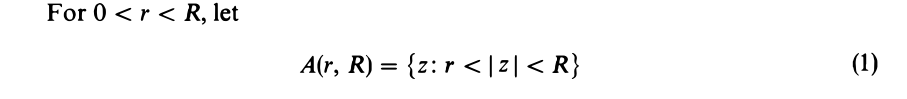
\includegraphics[width=\textwidth]{2-hw15-2025061123.png}
% \caption{}
\label{}
\end{figure}
\begin{figure}[H]
\centering
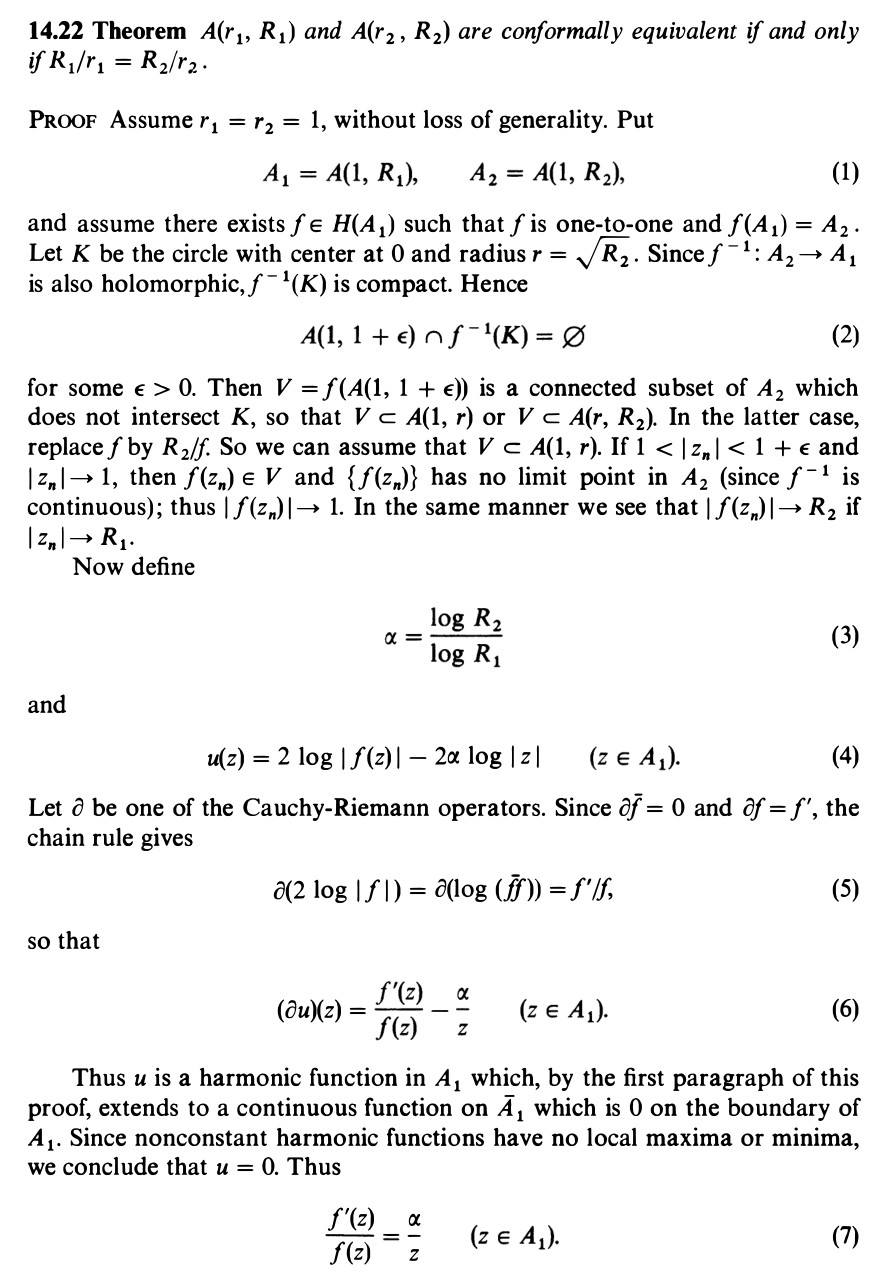
\includegraphics[width=\textwidth]{hw15-2025061123.png}
% \caption{}
\label{}
\end{figure}
\begin{figure}[H]
\centering
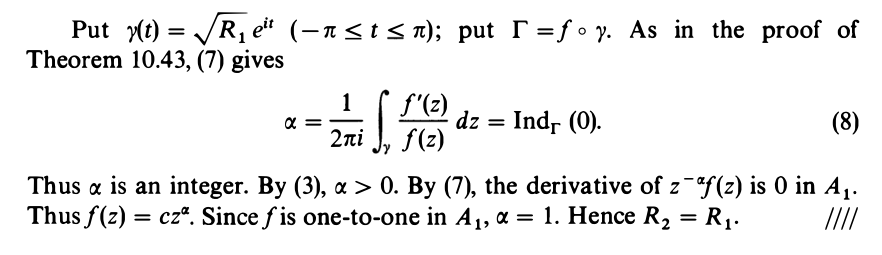
\includegraphics[width=\textwidth]{1-hw15-2025061123.png}
% \caption{}
\label{}
\end{figure}

\begin{exercise}
\begin{figure}[H]
\centering
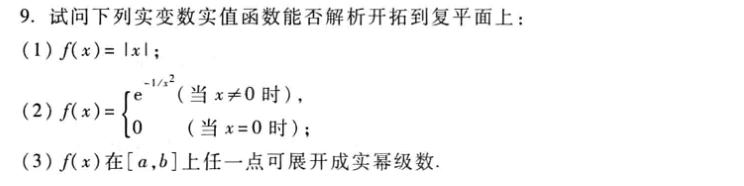
\includegraphics[width=\textwidth]{2-hw15-2025060920.png}
% \caption{}
\label{}
\end{figure}
\end{exercise}
\begin{figure}[H]
\centering
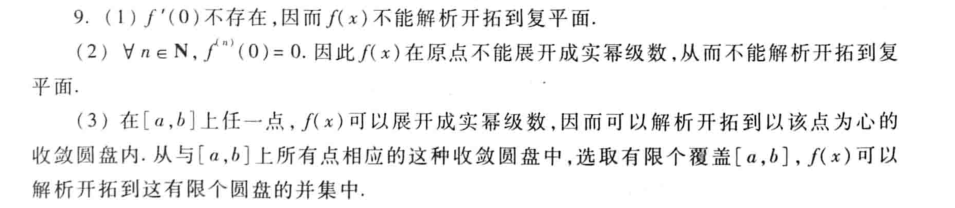
\includegraphics[width=\textwidth]{hw15-2025061011.png}
% \caption{}
\label{}
\end{figure}
